% !TeX spellcheck = en_US
% !TeX root = ../build/l2-state-tree-concept.tex
% !TeX TXS-program:compile = txs:///xelatex/[--shell-escape]






%%%%%%%%%%%%%%%%%%%%%%%%%%%%%%%%%%%%%%%%%%%%%%%%%%%%%%%%%%%%%%%%%%%%%%%%%%
\section{L2 State Tree Concept}




%%%%%%%%%%%%%%%%%%%%%%%%%%%%%%%%%%%%%%%%%%%%%%%%%%%%%%%%%%%%%%%%%%%%%%%%%%
\subsection{Introduction}

In this section, will be discussed the State Tree of Layer 2 within the zkEVM architecture. The main components of the zkEVM architecture in this section are: the \textbf{Prover}, the Prover's \textbf{HashDB} and the \textbf{Executor}.

In Ethereum, ensuring the accuracy of state changes resulting from the execution of transactions is crucial. Within the zkEVM context, the \textbf{zkEVM ROM} is a \textbf{zkASM program} designed to prove computations for stating the correct Layer 2 State transitions from a given a batch of L2 transactions. We might use multiple zkASM instructions to implement a single zkEVM opcode (in fact, this happens most of the times). Recall that the L2 State is organized as a Merkle Tree, being its root a cryptographic summary of the current state data referred to as the \textbf{State Root}. Hence, the \textbf{ROM} must have the capability to \textbf{correctly} execute CRUD (Create, Read, Update, and Delete) operations on the Merkle Tree representing the current state.



\subsection{Introduction to the Storage State Machine}

In the zkEVM, a secondary State Machine known as the \textbf{Storage State Machine} has been implemented. This machine is specifically designed to generate an execution trace, providing evidence for the creation, reading, updating, and deletion of L2 state data. For example, when we need to retrieve a value from the tree, it's essential to obtain a set of nodes from the tree, referred to as the Merkle proof, ensuring the accuracy of the read state value. Similarly, any operation that modifies the tree must provide proof that the tree modification is executed correctly. After processing the last L2 transaction in a batch, the resulting root will be the new state root.


Let's provide specific illustrative examples (Figure \ref{fig:examples}) showcasing CRUD operations on the L2 State, being the Storage State Machine responsible for providing proof of their validity:

\begin{figure}[H]
\centering
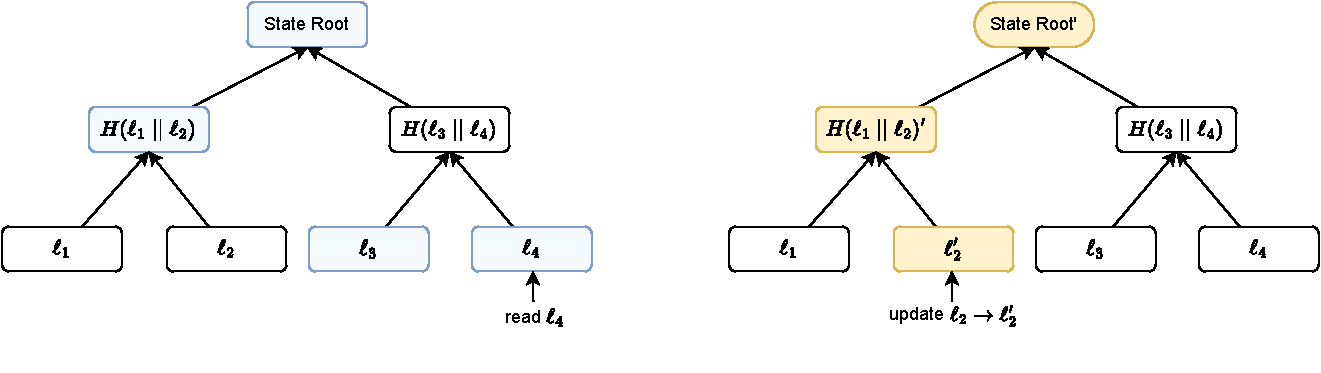
\includegraphics[width=0.9\columnwidth]{\trainingsectiondir/figures/read-write-merkle-tree.drawio}
\caption{Read proof for the leaf $\ell_4$ (left) and update of the leaf $\ell_2$ to a new value $\ell_4'$ (right).}
\label{fig:examples}
\end{figure}

In the left figure, the objective is to read the information of the fourth leaf ($\ell_4$). Suppose we are conducting a transaction, and $\ell_4$ represents the balance of the account initiating the transaction. In the process of reading this leaf, it is crucial to verify its inclusion in the current state at the specified position (which will be deterministically computed from some unique properties of the data being stored, such as the account address or the type of data). The Storage State Machine comes into play by generating an execution trace, and the boxes highlighted in blue must be supplied to it. These blue boxes enable the Storage State Machine to validate that the root it computes aligns with the State Root that we have.

In the right figure, we examine a scenario where a leaf is updated, resulting in a change in its value and, consequently, a modification of the State Root. Specifically, all the yellow boxes in the figure are affected as they incorporate information from the updated leaf $\ell_2'$. The Storage State Machine is once again employed to generate an execution trace, ensuring the accuracy of all tree modifications. By following the same procedure, the consistency of State Roots is verified to confirm that the changes have been accurately executed.

All the essential hashes required for computing execution traces are stored in the \textbf{HashDB}. During the execution of the L2 State's related zkEVM opcodes (like for example \texttt{:SSTORE} or  \texttt{:SLOAD}), the Storage State Machine's Executor consistently retrieves values from the HashDB and use them in order to construct the corresponding execution traces. The HashDB contains all the hashes (i.e., all the nodes) of the Merkle tree of the L2 state. In Figure \ref{fig:executor-db-interaction} we can observe how the Executor process works.

\begin{figure}[H]
\centering
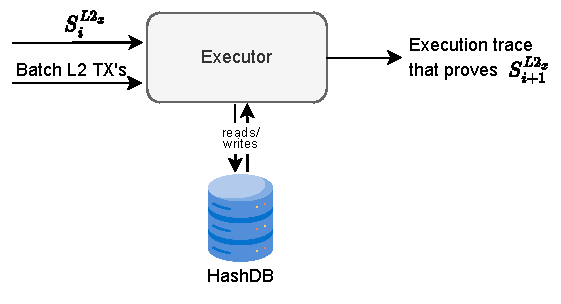
\includegraphics[width=0.62\columnwidth]{\trainingsectiondir/figures/executor-diagram.drawio}
\caption{Executor Proving the current State by Interacting with the HashDB to retrieve the corresponding Merkle Proofs to fill the execution trace.}
\label{fig:executor-db-interaction}
\end{figure}


It's important noting that the Merkle tree utilized in the Polygon zkEVM is a binary Sparse Merkle Tree (SMT), distinguishing itself from the Merkle tree in the L1 EVM, which is a completely different hexary structure.


